\documentclass{scrartcl}

\usepackage[utf8]{inputenc}
\usepackage[T1]{fontenc}
\usepackage{lmodern}
\usepackage[english]{babel}
\usepackage{amsmath}
\usepackage{graphicx}
\usepackage{caption}	
\usepackage{subcaption}	 
\usepackage{hyperref}
\usepackage[parfill]{parskip}
\usepackage{hhline}
\usepackage{subcaption}

\title{Neuroprosthetics - Exercise 6}
\author{Alexander Koenig}
\date{21. December 2019}

\begin{document}
\maketitle

\section{Calculate the Potential Field}

The potential resulting from a current point source is calculated with equation \ref{eq:potential}. The potential is directly proportional to the current. A visualization of the potential field for a $50 \mu m$ by $50 \mu m$ slice at a distance of $10 \mu m$ is displayed in figure \ref{fig:potential}. The current is $I=1mA$ and the electrical conductivity of the medium is $\rho = 300 \Omega cm$. 

\begin{equation} \label{eq:potential}
\Phi=\frac{\rho}{4 \pi} \cdot \frac{I}{r}
\end{equation}

\begin{figure}[h]
	\centering
	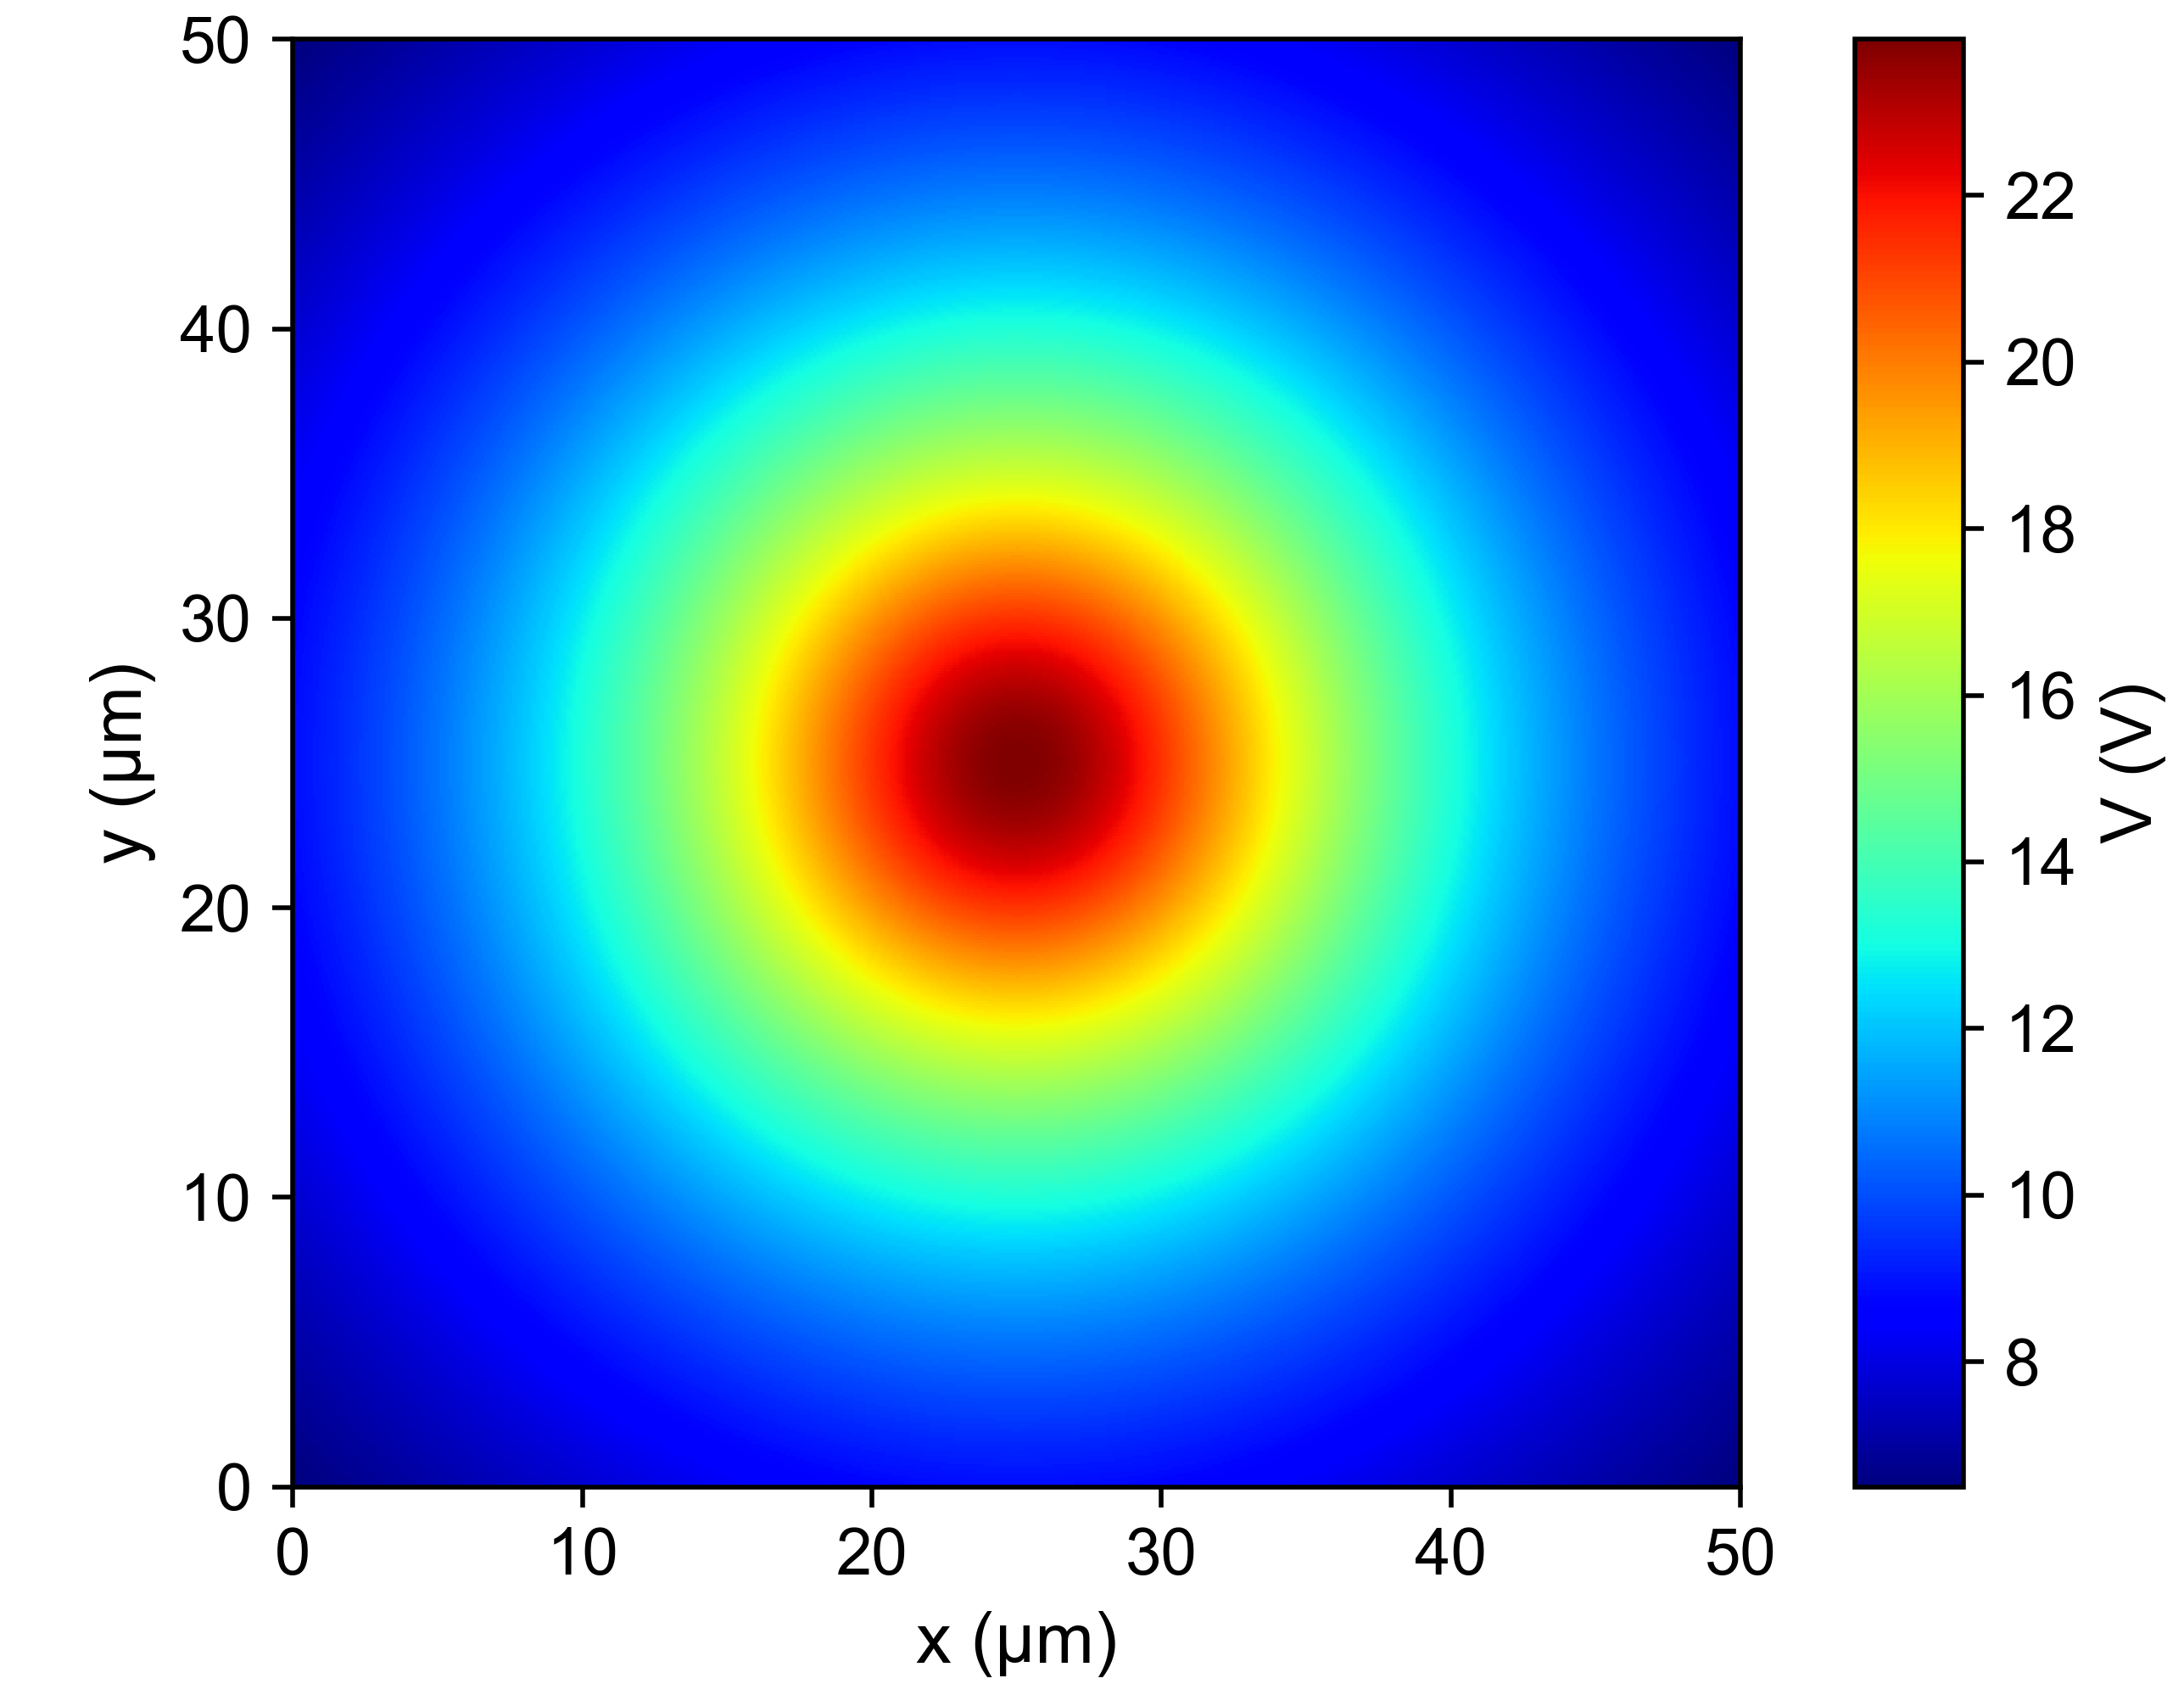
\includegraphics[width=0.8\textwidth]{figures/potential_processed}
	\caption{Potential from current source}
	\label{fig:potential}
\end{figure}

Figure \ref{fig:potential_and_derivatives} shows the potential field, the electric field and the activation function in a $50 \mu m$ piece of axon positioned $10 \mu m$ from the current point source. The three graphs are plotted for an electrode current of $1 mA$ and $-1mA$.

From the first two graphs, it becomes clear that the external potential at the axon is positive if the current source is positive (direct proportionality). The potential follows a non-linear profile and reaches its maximum/minimum at the point where the current source is closest to the axon, at $25 \mu m$.

The electric field is defined as the negative first spatial derivative of the potential (in absence of a magnetic potential). Hence the electric field follows the displayed trajectory, with two peaks/throughs where the change of the potential is smallest/greatest. The electric field is zero at the point where the potential reaches its maximum/minimum.

The activation function is calculated as the second derivative of the external potential. It is evident from the plot that the activation functions for both currents have their maximum/minimum at the point where the potential reaches its minimum/maximum. The activation function describes the activation of the neuron due to an external potential. 

\begin{figure}[h]
	\centering
	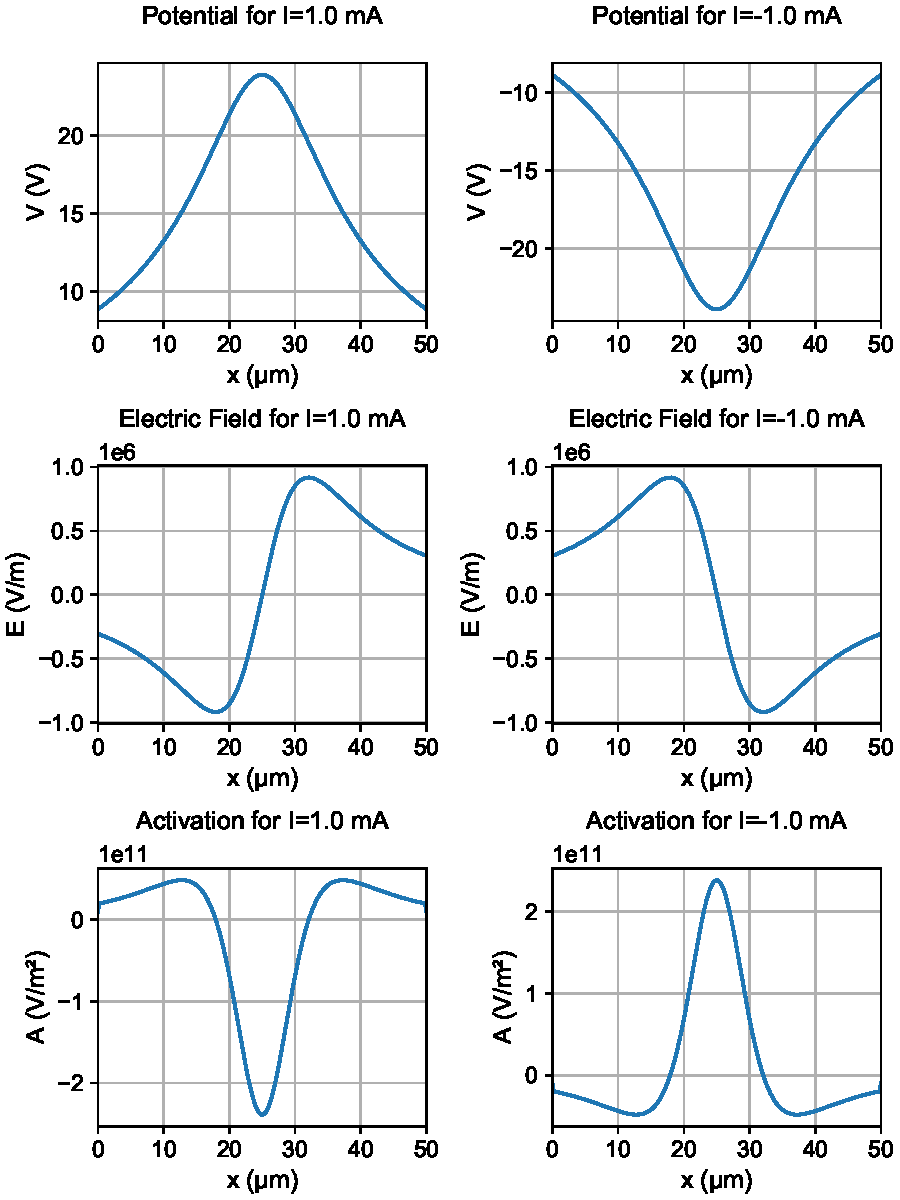
\includegraphics[width=0.95\textwidth]{figures/potential_and_derivatives}
	\caption{Potential, electric field and activation function for different currents}
	\label{fig:potential_and_derivatives}
\end{figure}

\section{Calculate a Neuron Model}
The model from exercise 5 is enhanced to model the influence of an external potential on the axon. The axon is positioned as in section 1 and simulations are run with different stimulation sequences. The phase duration of all pulses is 1ms. 

\begin{itemize}
	\item Figure \ref{fig:sim1} shows that the current pulse is too weak to elicit an action potential. The positive activation only lifts the membrane potential to approximately 1.6mV and does not reach the firing threshold. The compartments around the peak experience a negative activation and hence show a darker shade of blue in the plot. There is a small undershoot of the membrane potential after the current pulse due to the slow closing of the potassium channels. 
	\item Figure \ref{fig:sim2} shows the clear formation of an action potential. The current pulse of -1mA results in a strong enough neuronal activation to lift the membrane potential above the firing threshold. The signal then propagates linearly in both directions, like in the previous exercise. 
	\item Figure \ref{fig:sim3} shows a similar situation as in figure \ref{fig:sim1}. The first phase of the bi-phasic current pulse can not lift the membrane potential above the threshold and no action potential can form. The simulation differs from the simulation in figure \ref{fig:sim1} in that the rise of the membrane potential is much shorter as the second phase of the pulse immediately reduces the membrane potential with its negative activation (positive potential leads to negative activation in the middle compartments of the axon). 
	\item Figure \ref{fig:sim4} shows that the formation of an action potential is possible using a bi-phasic current pulse if the first pulse is strong enough.
	\item Figure \ref{fig:sim5} shows that a positive current pulse reduces the membrane potential in the middle compartments due to its negative activation. The membrane potential in the outer compartments rises, but at approximately 0.3mV it is far from the firing threshold. No action potentials can be elicited. 
	\item Figure \ref{fig:sim6} demonstrates that if a positive current pulse is strong enough multiple action potentials can be elicited. Approximately at compartments 20 and 80, the membrane potential is lifted above the firing threshold by the positive parts of the activation function. Two action potentials form from these two points and a third one is elicited in the middle compartments at roughly 15ms. The outer action potentials travel towards the inner one and destructively interfere because the neighboring compartments of the compartment in which the action potentials meet are still in their absolute refractory period.
\end{itemize}

\newpage
\begin{figure}[h]
	\centering
	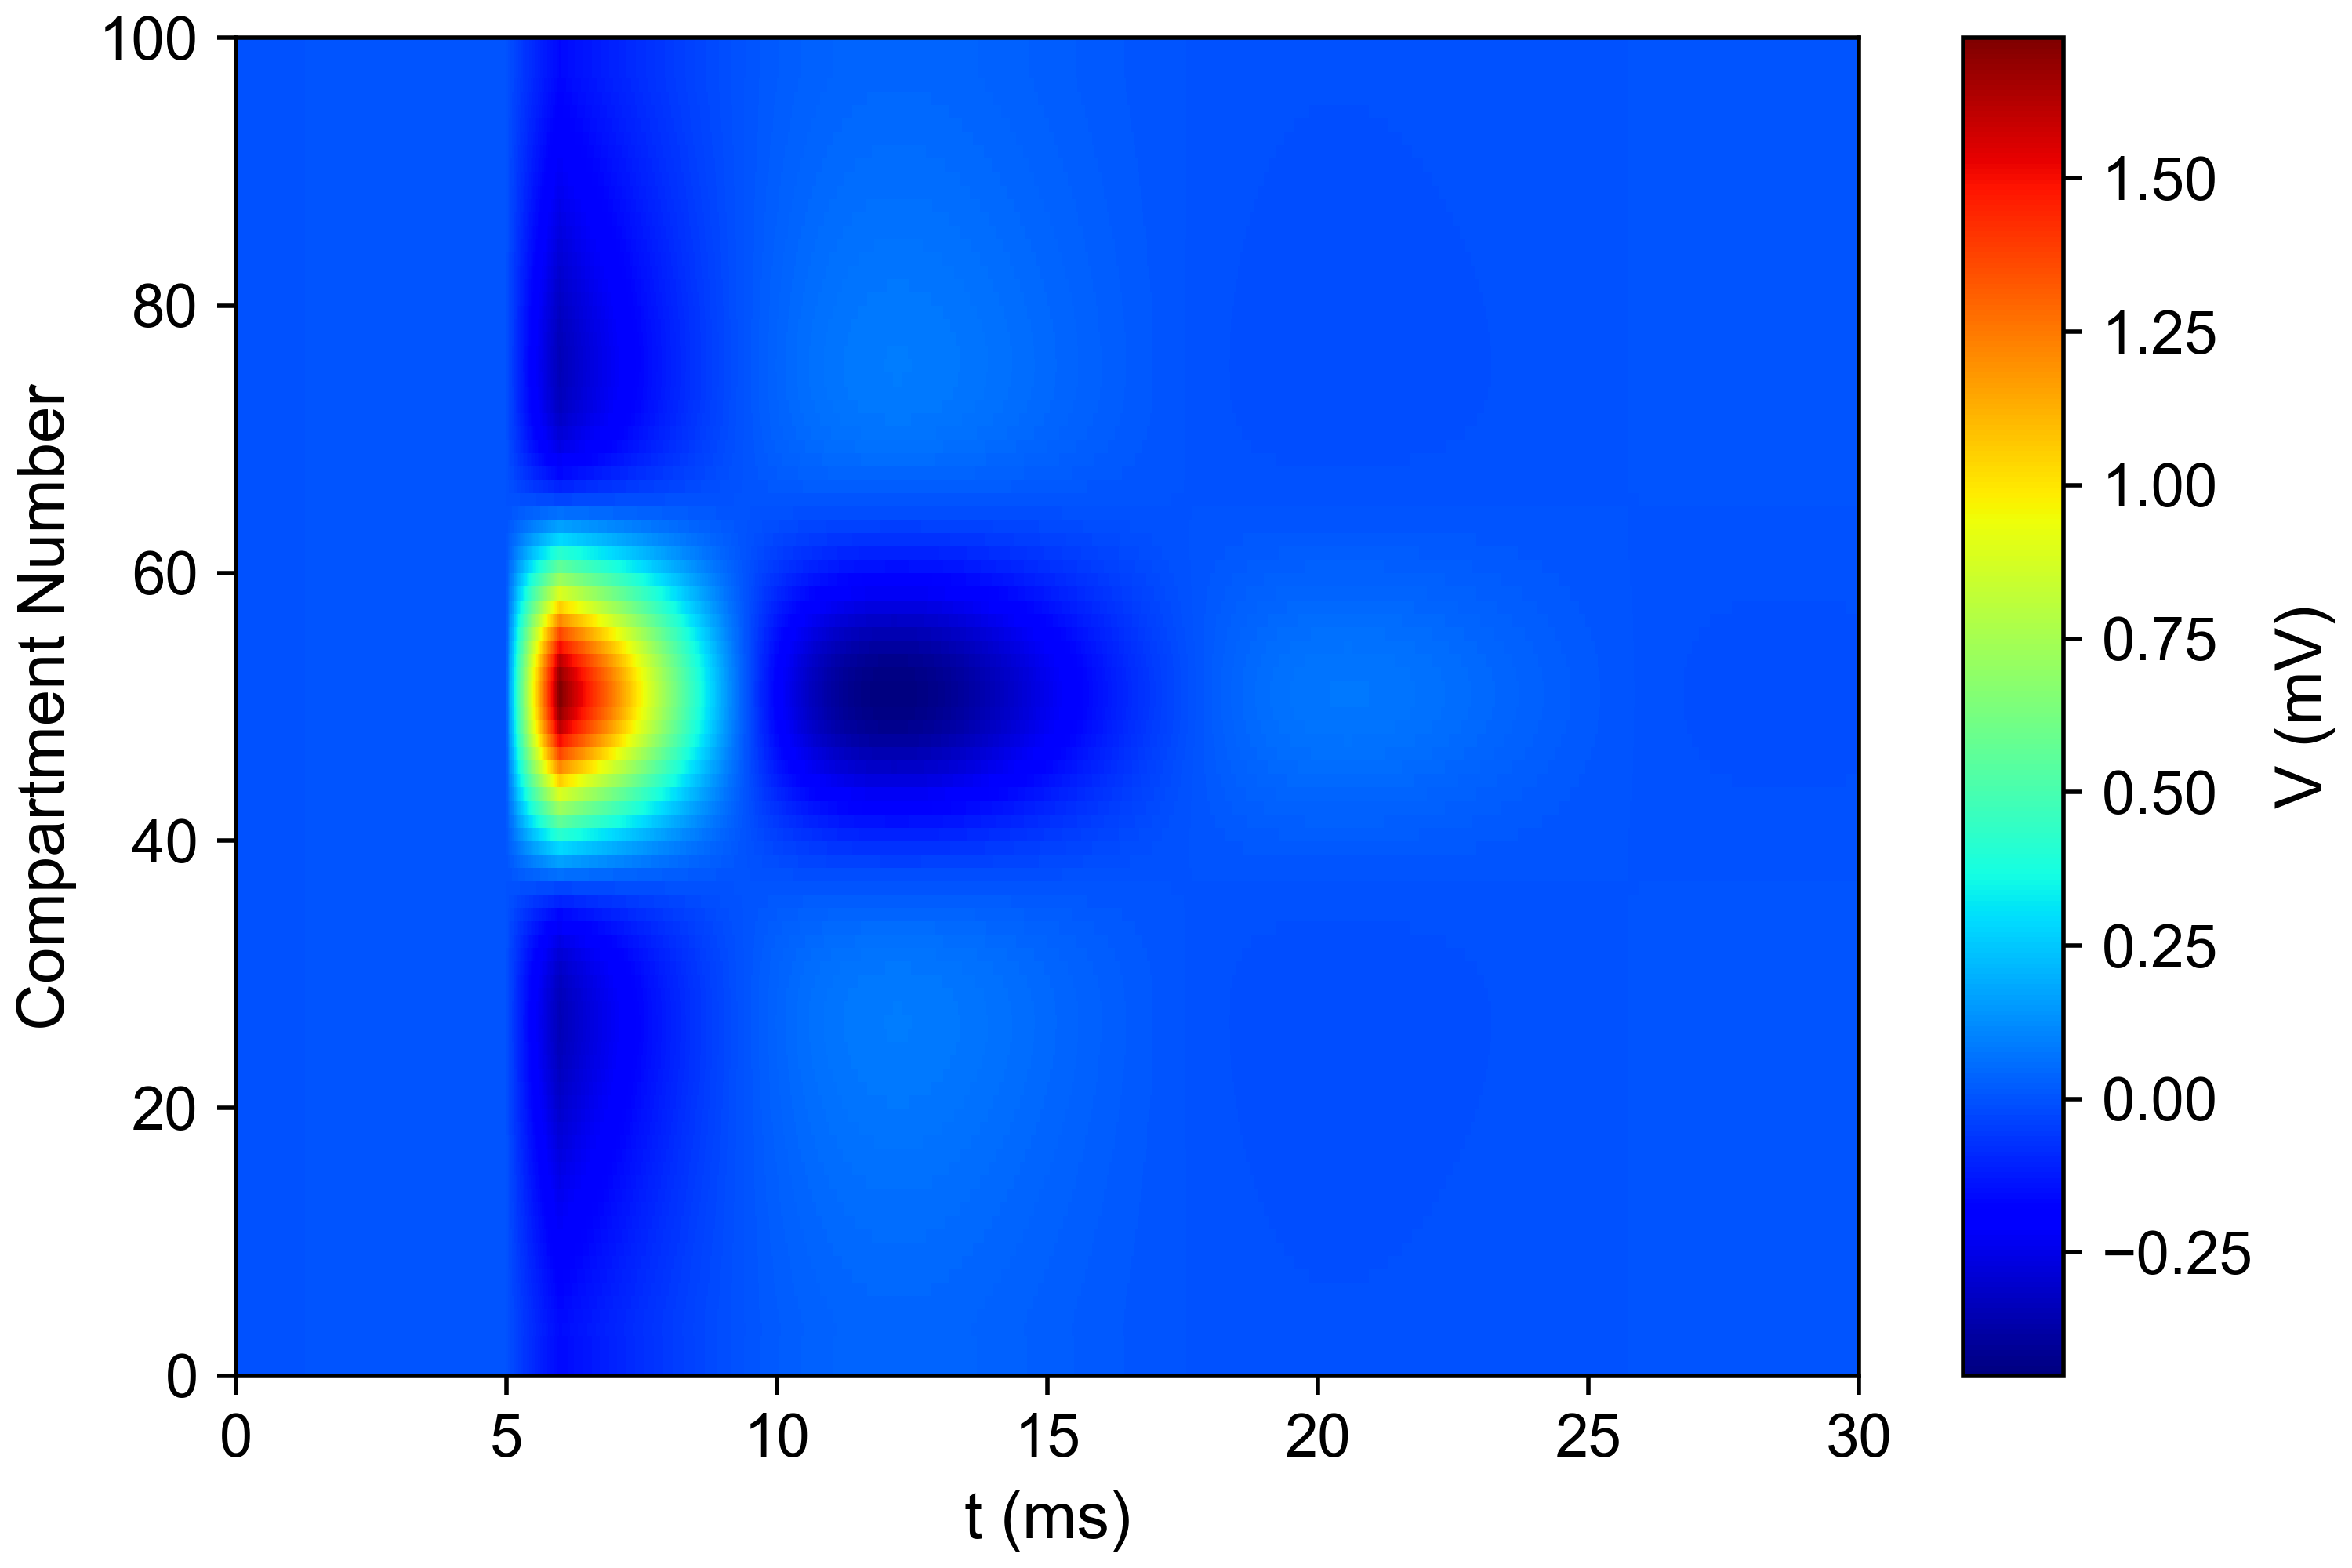
\includegraphics[width=0.9\textwidth]{figures/potential_SimulationType.mono_amp-0.00025.png}
	\caption{Stimulation type: mono-phasic, Current: -0.25mA}
	\label{fig:sim1}
\end{figure}
\begin{figure}[h!]
	\centering
	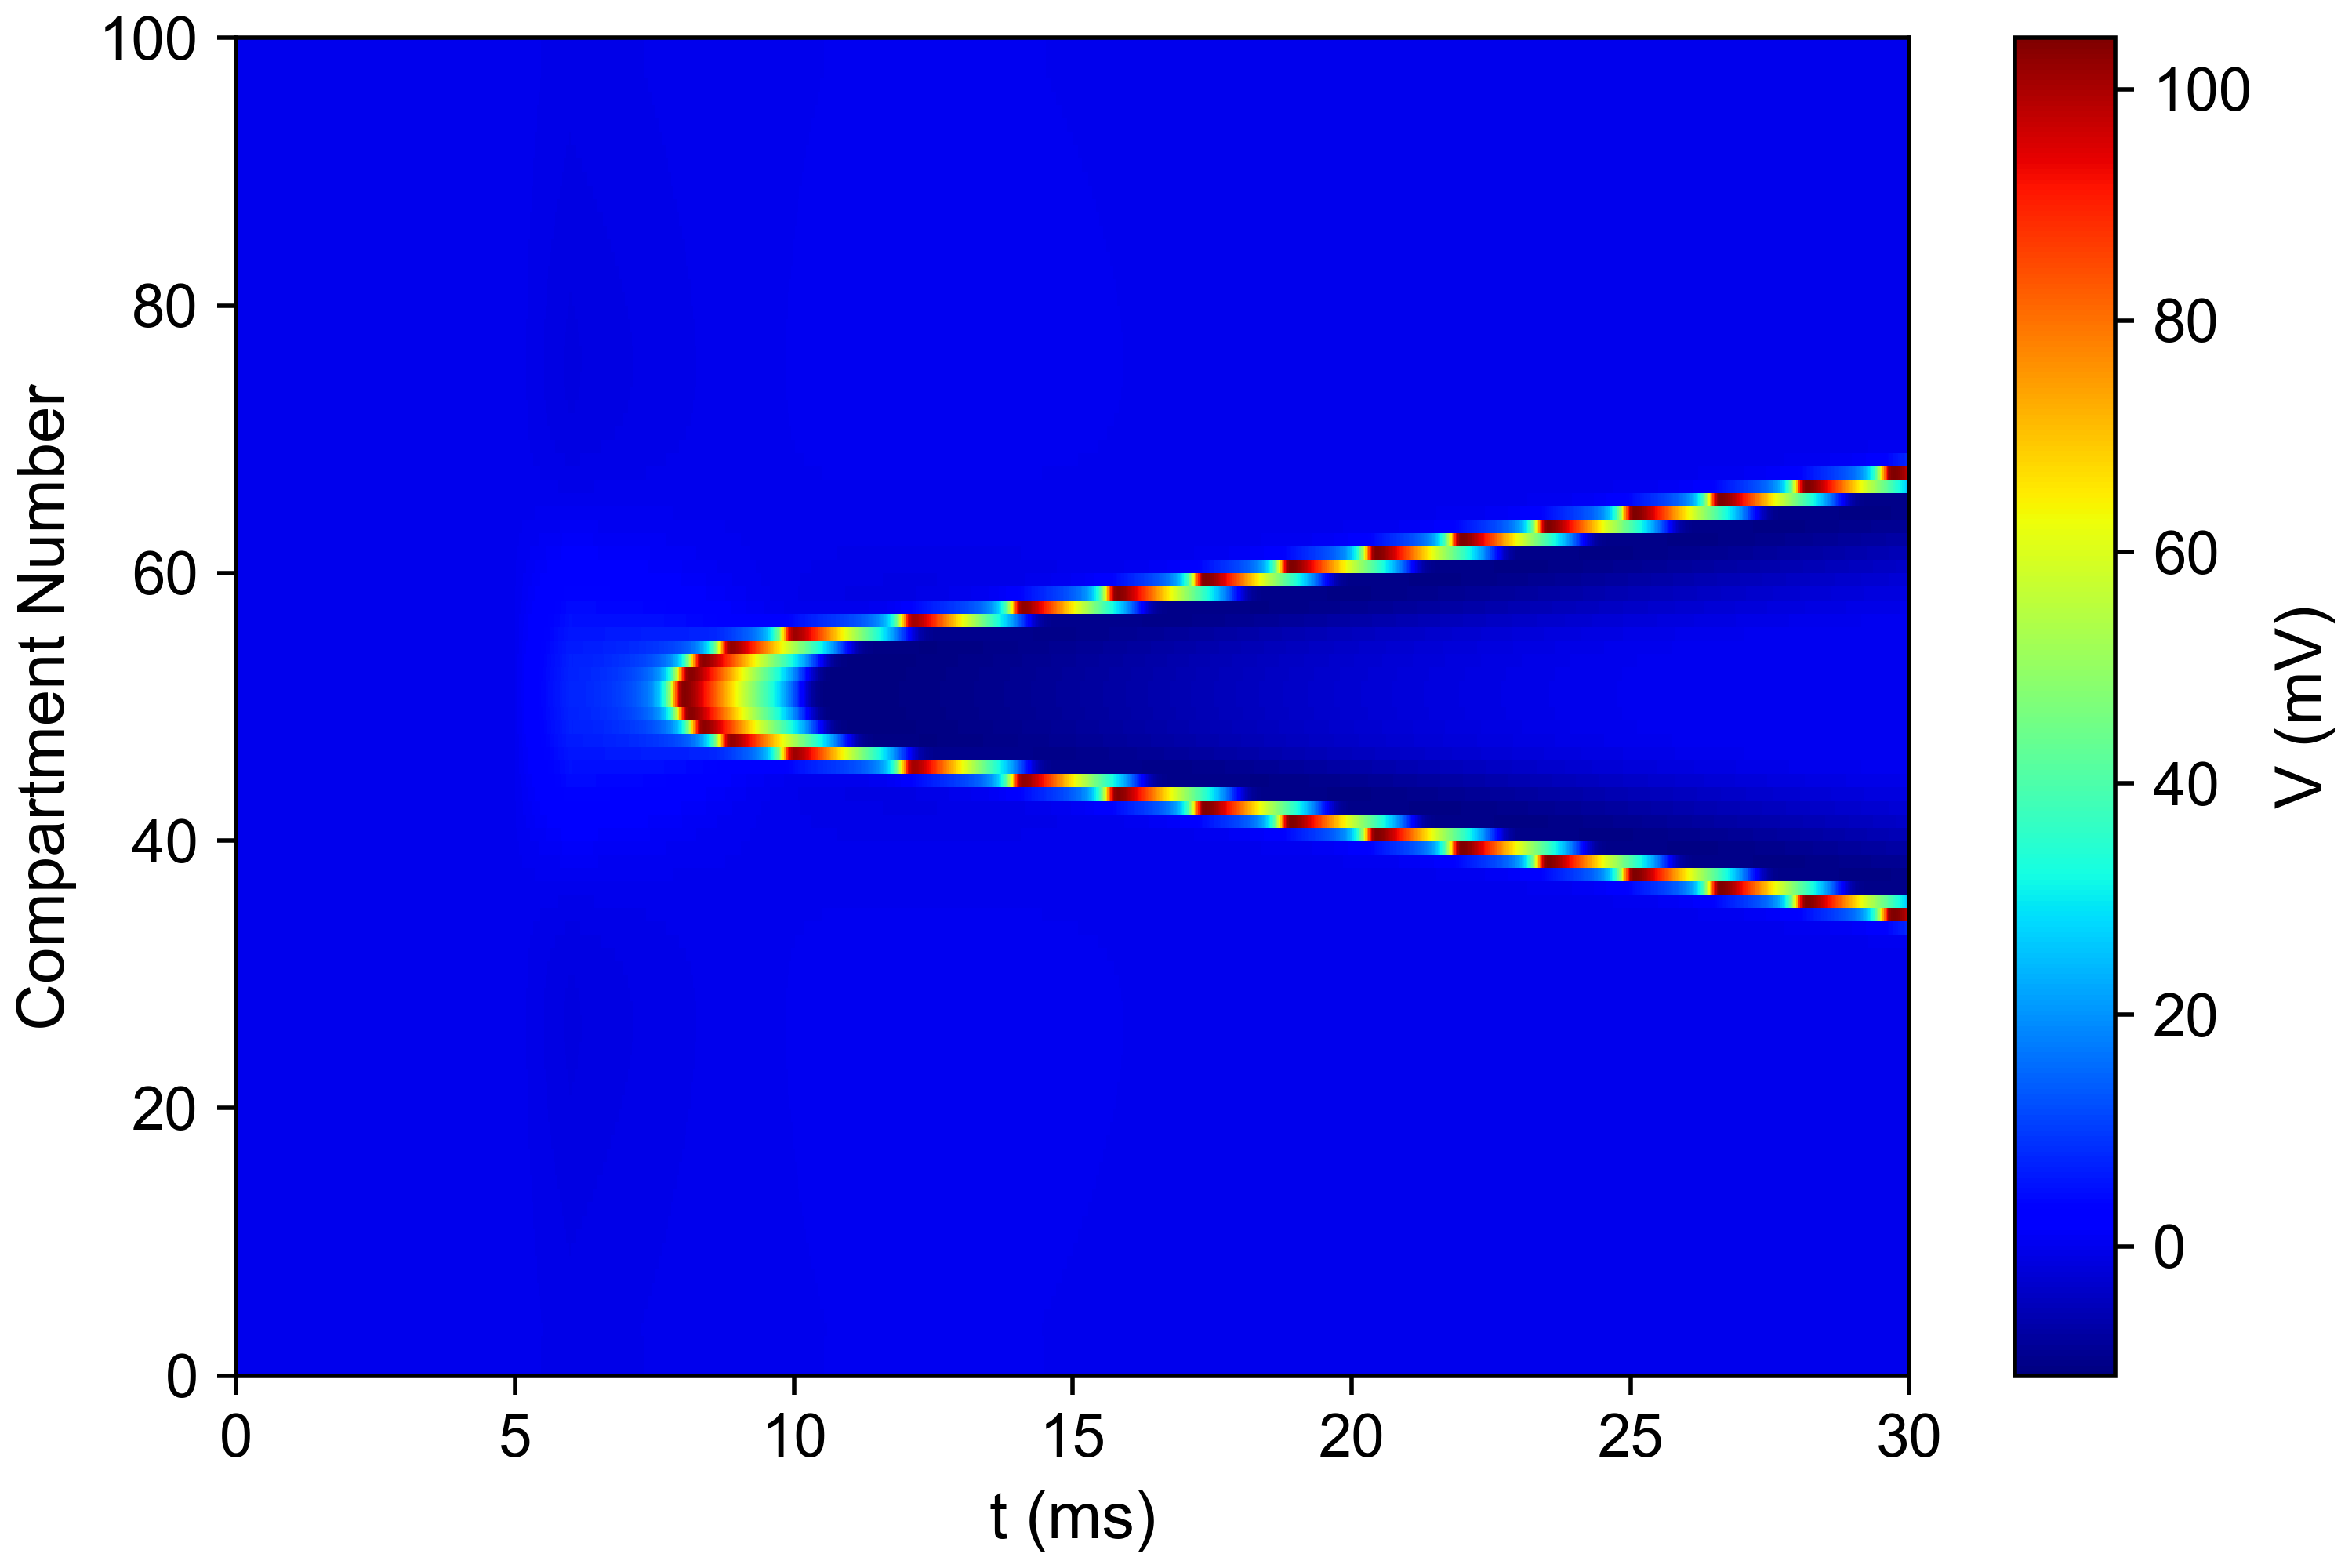
\includegraphics[width=0.9\textwidth]{figures/potential_SimulationType.mono_amp-0.001.png}
	\caption{Stimulation type: mono-phasic, Current: -1mA}
	\label{fig:sim2}
\end{figure}

\newpage
\begin{figure}[h]
	\centering
	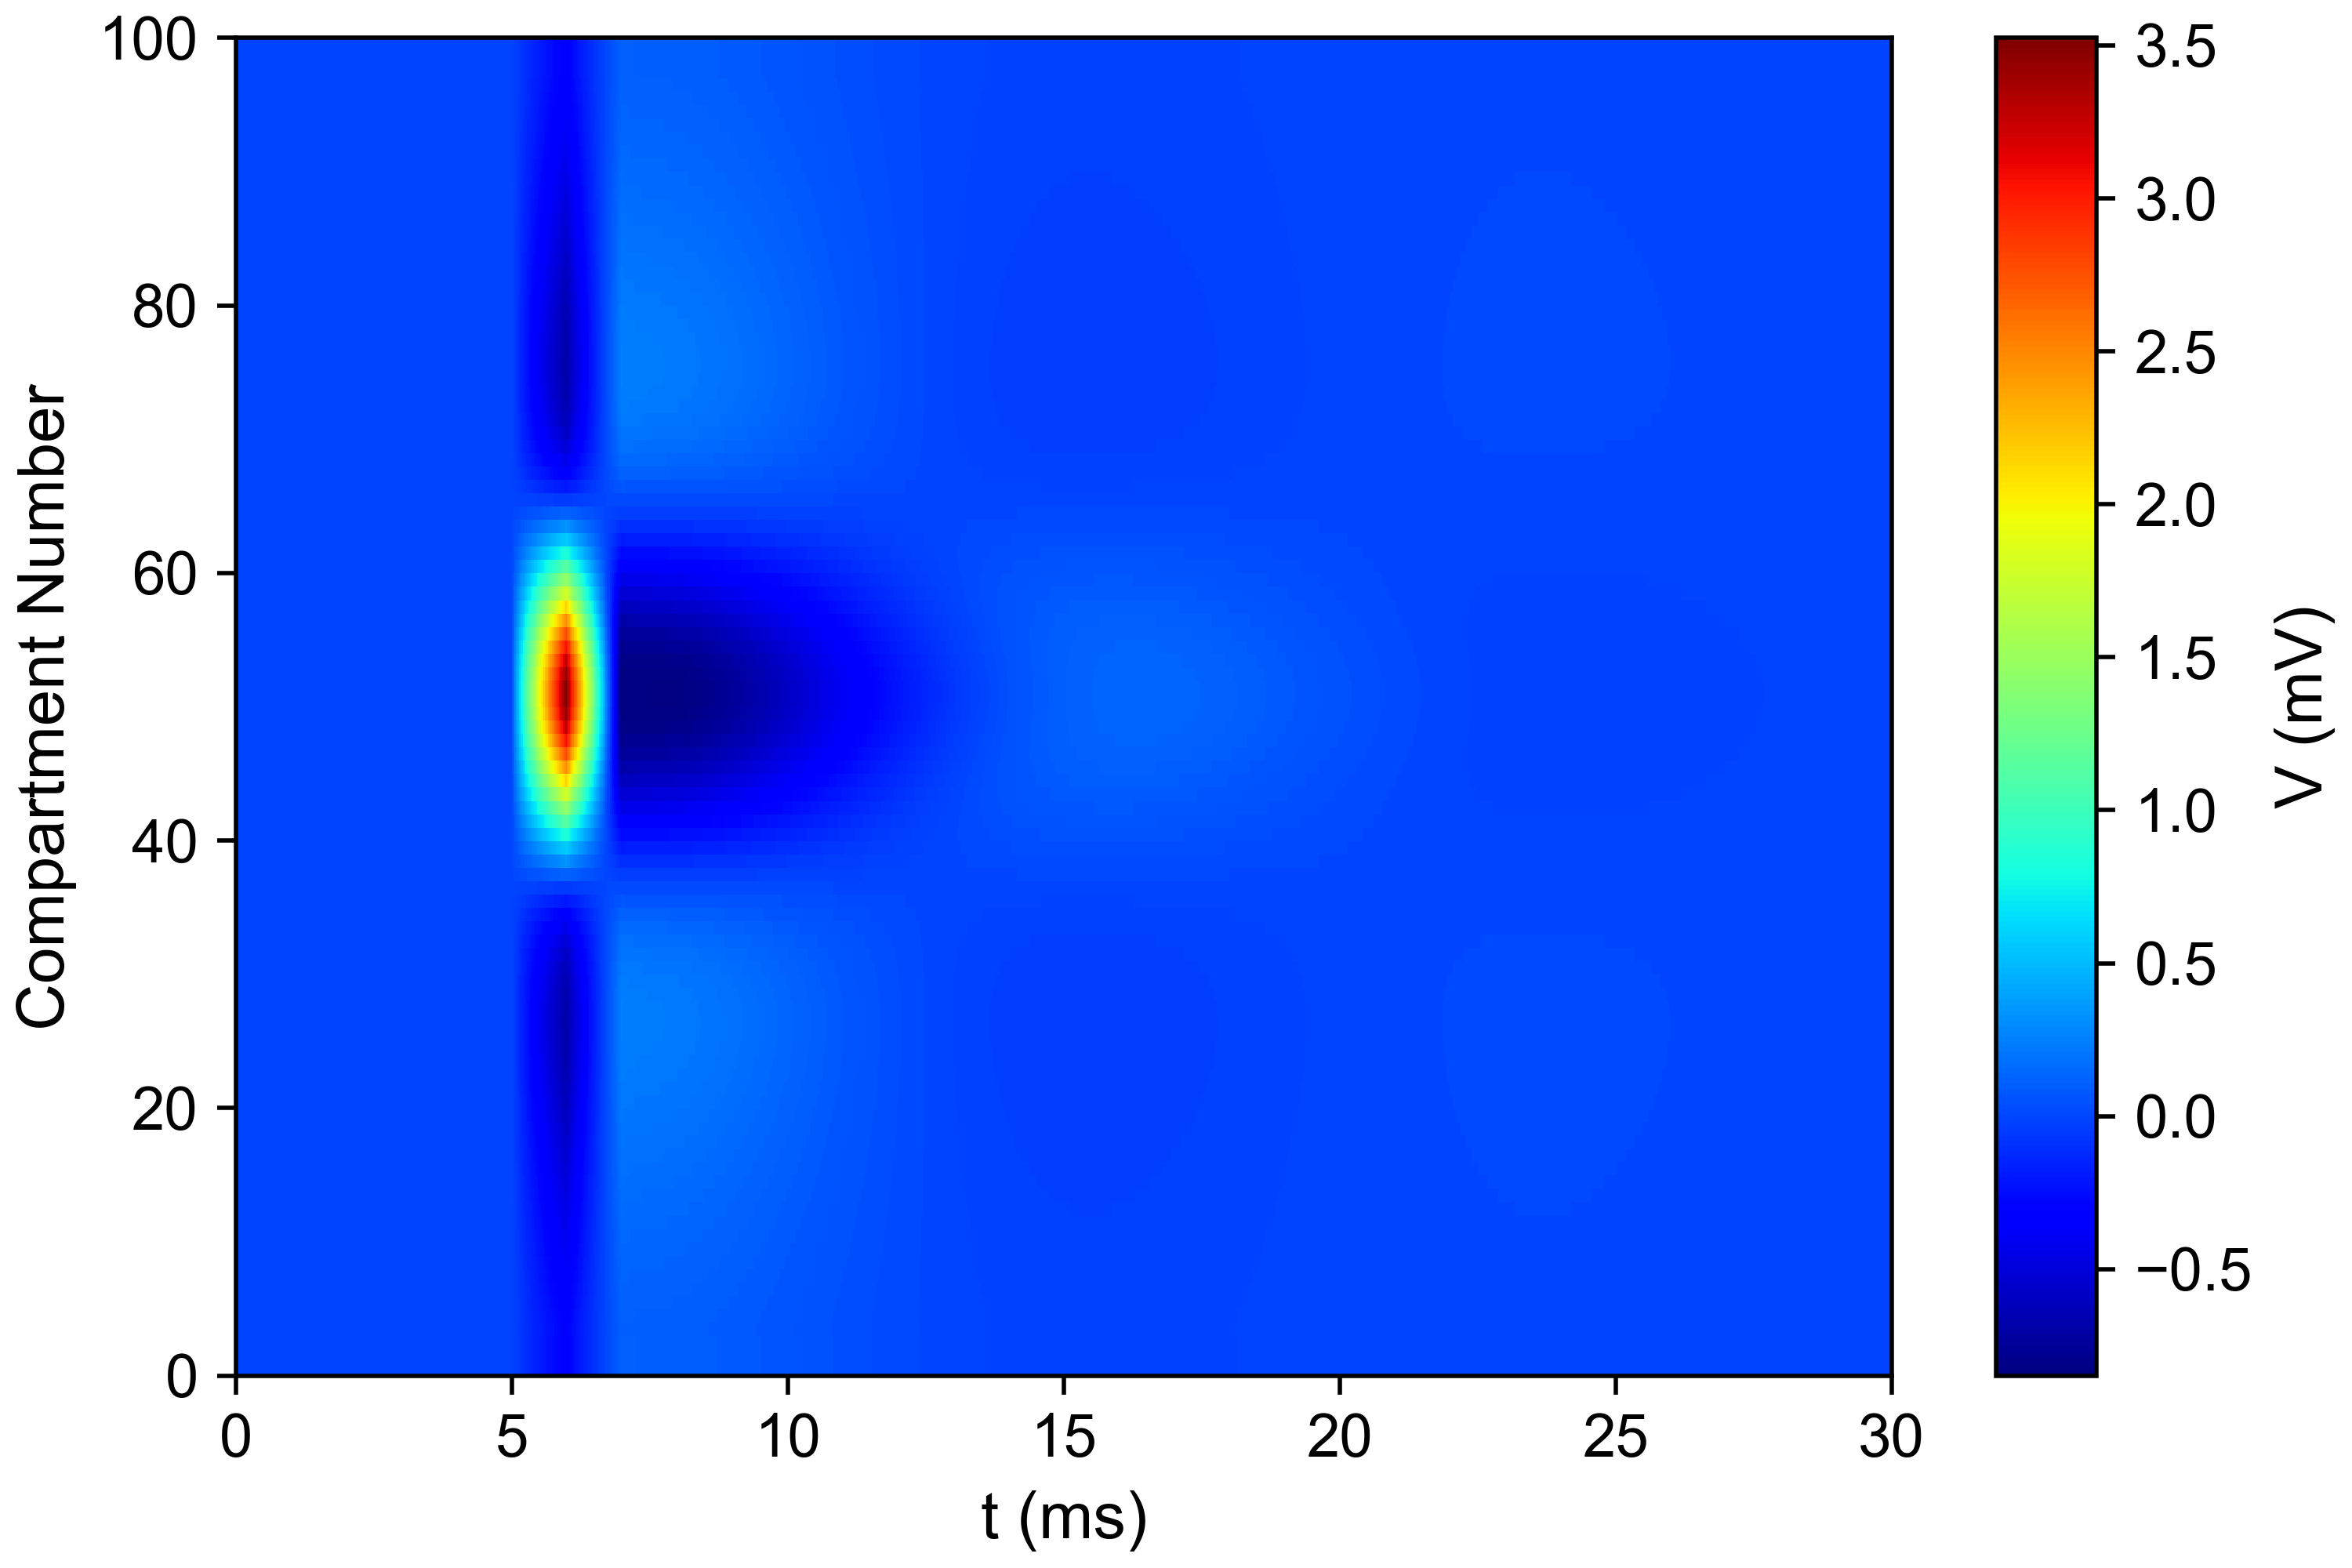
\includegraphics[width=0.9\textwidth]{figures/potential_SimulationType.bi_amp0.0005.png}
	\caption{Stimulation type: bi-phasic, Current amplitude: 0.5mA}
	\label{fig:sim3}
\end{figure}
\begin{figure}[h!]
	\centering
	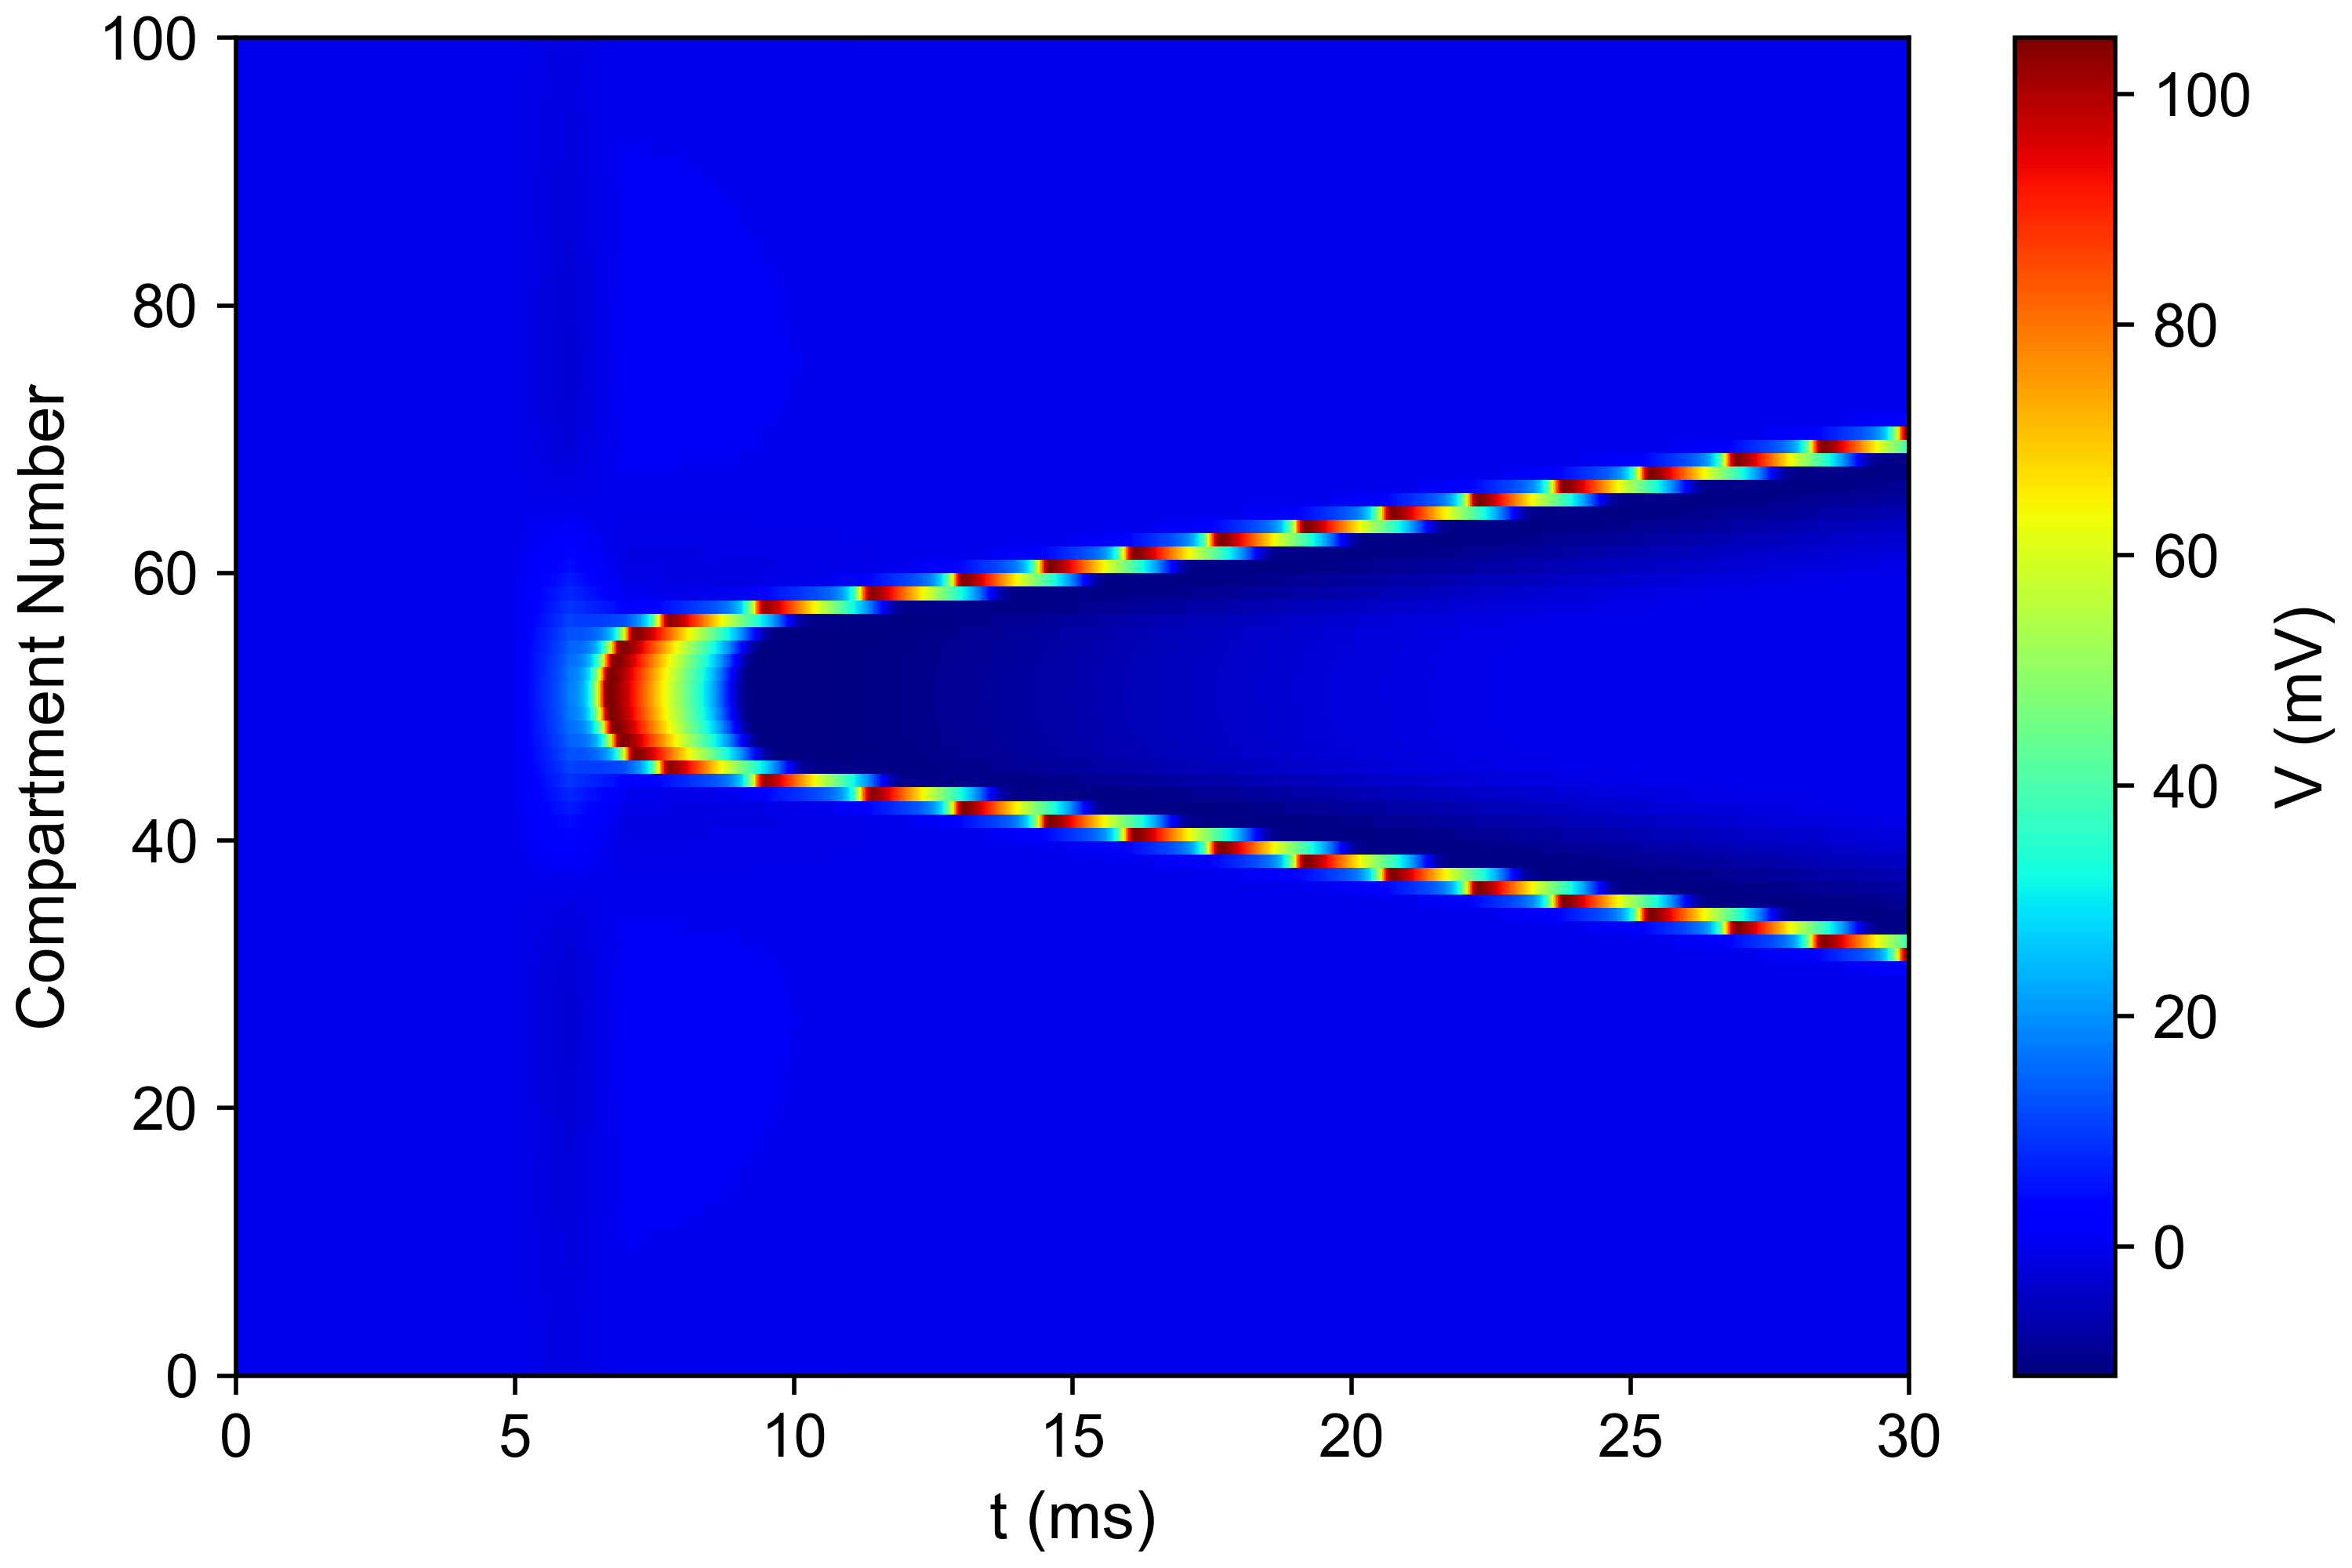
\includegraphics[width=0.9\textwidth]{figures/potential_SimulationType.bi_amp0.002.png}
	\caption{Stimulation type: bi-phasic, Current amplitude: 2mA}
	\label{fig:sim4}
\end{figure}

\newpage
\begin{figure}[h]
	\centering
	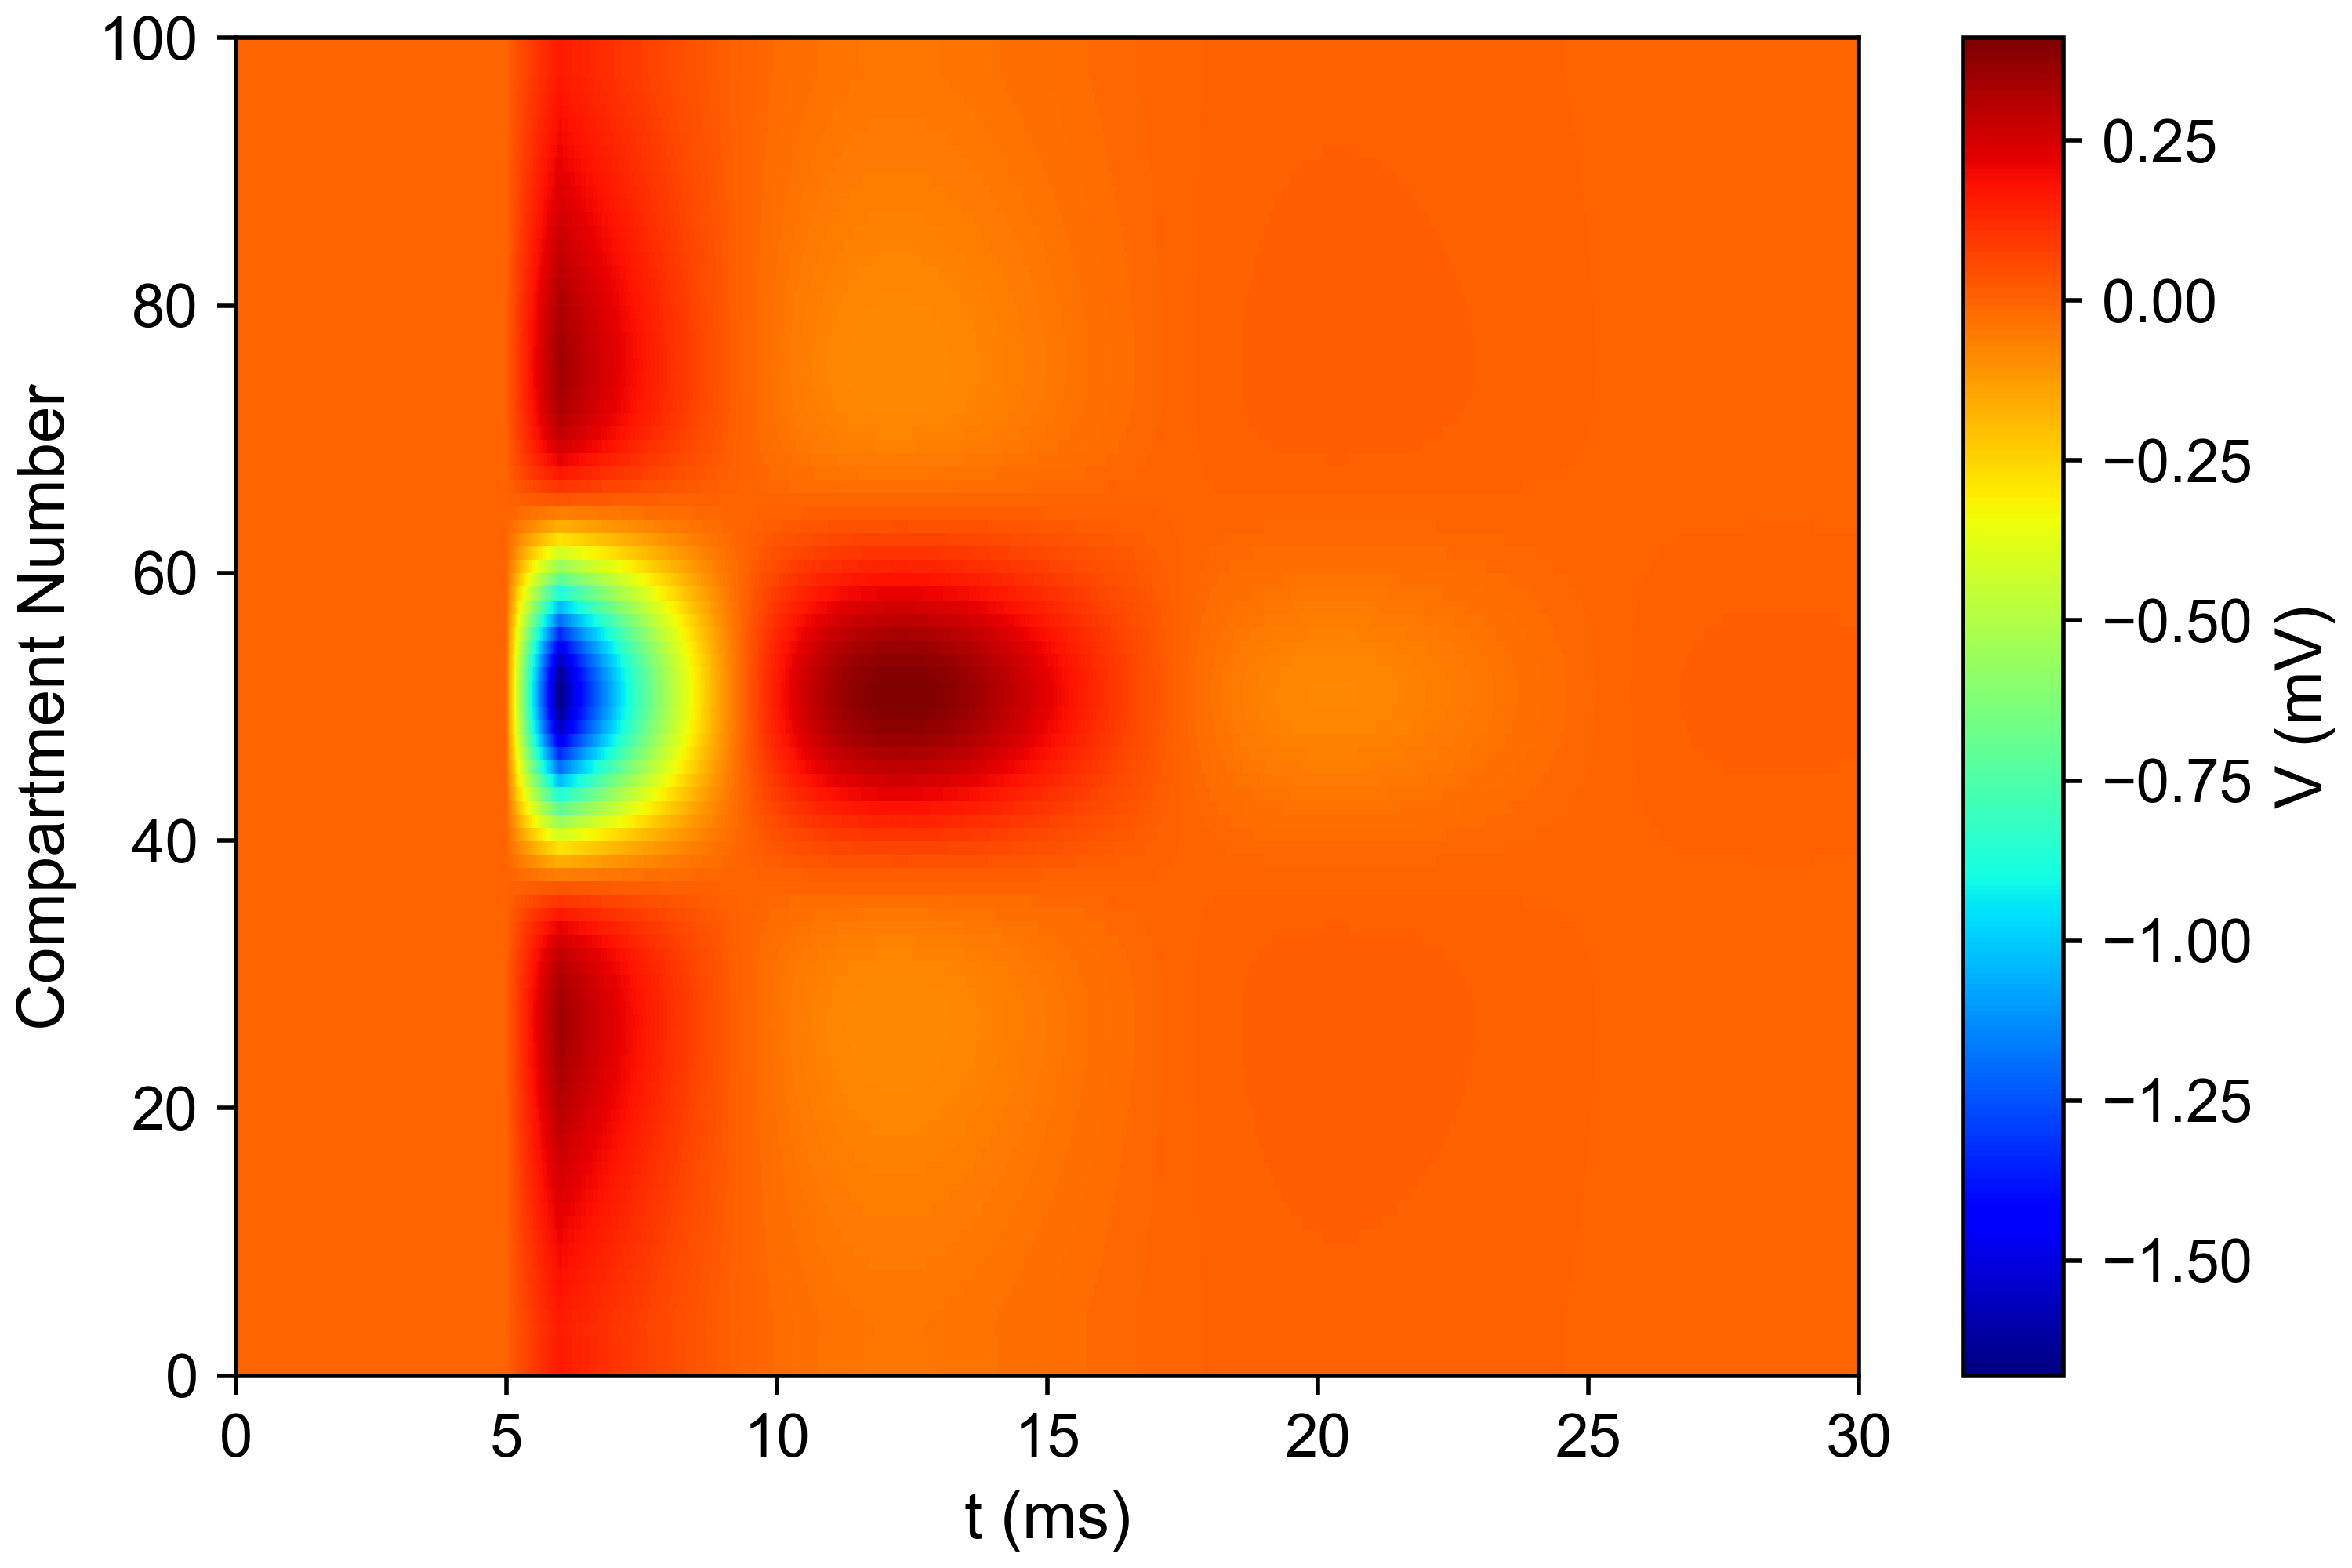
\includegraphics[width=0.9\textwidth]{figures/potential_SimulationType.mono_amp0.00025.png}
	\caption{Stimulation type: mono-phasic, Current: 0.25mA}
	\label{fig:sim5}
\end{figure}
\begin{figure}[h!]
	\centering
	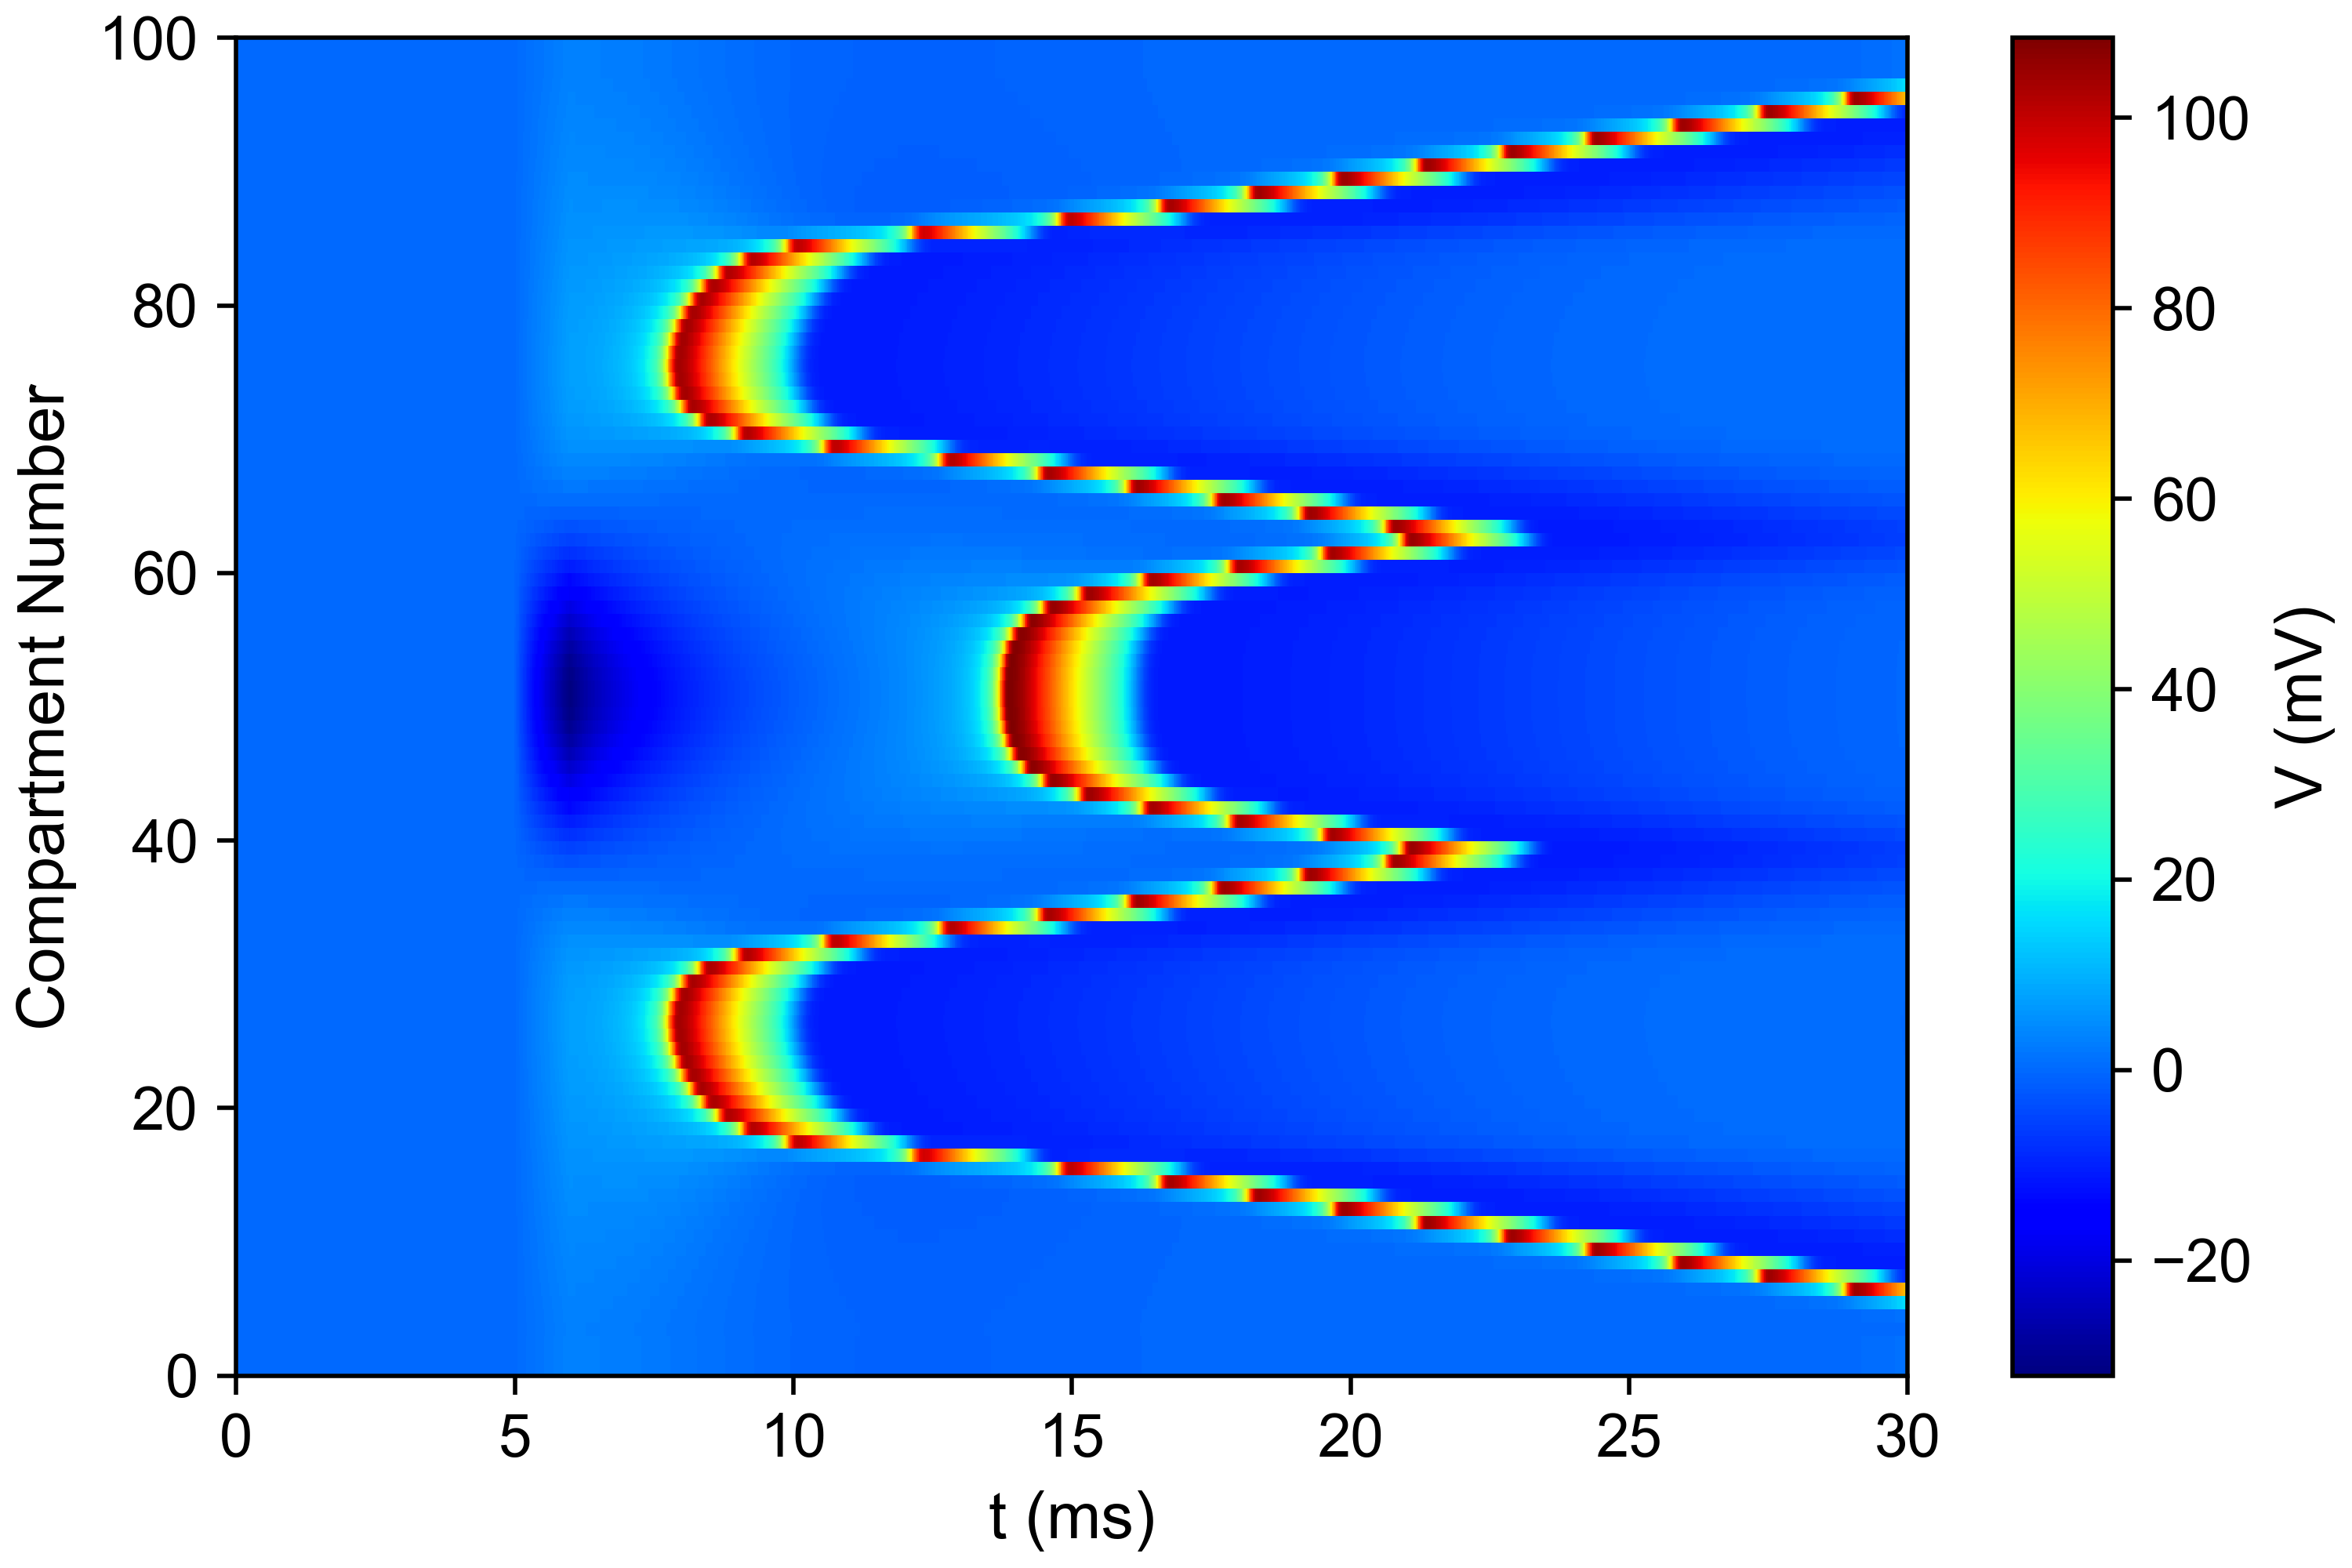
\includegraphics[width=0.9\textwidth]{figures/potential_SimulationType.mono_amp0.005.png}
	\caption{Stimulation type: mono-phasic, Current: 5mA}
	\label{fig:sim6}
\end{figure}
\end{document}